% Options for packages loaded elsewhere
\PassOptionsToPackage{unicode}{hyperref}
\PassOptionsToPackage{hyphens}{url}
%
\documentclass[
]{article}
\usepackage{amsmath,amssymb}
\usepackage{lmodern}
\usepackage{iftex}
\ifPDFTeX
  \usepackage[T1]{fontenc}
  \usepackage[utf8]{inputenc}
  \usepackage{textcomp} % provide euro and other symbols
\else % if luatex or xetex
  \usepackage{unicode-math}
  \defaultfontfeatures{Scale=MatchLowercase}
  \defaultfontfeatures[\rmfamily]{Ligatures=TeX,Scale=1}
\fi
% Use upquote if available, for straight quotes in verbatim environments
\IfFileExists{upquote.sty}{\usepackage{upquote}}{}
\IfFileExists{microtype.sty}{% use microtype if available
  \usepackage[]{microtype}
  \UseMicrotypeSet[protrusion]{basicmath} % disable protrusion for tt fonts
}{}
\makeatletter
\@ifundefined{KOMAClassName}{% if non-KOMA class
  \IfFileExists{parskip.sty}{%
    \usepackage{parskip}
  }{% else
    \setlength{\parindent}{0pt}
    \setlength{\parskip}{6pt plus 2pt minus 1pt}}
}{% if KOMA class
  \KOMAoptions{parskip=half}}
\makeatother
\usepackage{xcolor}
\usepackage[margin=1in]{geometry}
\usepackage{graphicx}
\makeatletter
\def\maxwidth{\ifdim\Gin@nat@width>\linewidth\linewidth\else\Gin@nat@width\fi}
\def\maxheight{\ifdim\Gin@nat@height>\textheight\textheight\else\Gin@nat@height\fi}
\makeatother
% Scale images if necessary, so that they will not overflow the page
% margins by default, and it is still possible to overwrite the defaults
% using explicit options in \includegraphics[width, height, ...]{}
\setkeys{Gin}{width=\maxwidth,height=\maxheight,keepaspectratio}
% Set default figure placement to htbp
\makeatletter
\def\fps@figure{htbp}
\makeatother
\setlength{\emergencystretch}{3em} % prevent overfull lines
\providecommand{\tightlist}{%
  \setlength{\itemsep}{0pt}\setlength{\parskip}{0pt}}
\setcounter{secnumdepth}{-\maxdimen} % remove section numbering
\ifLuaTeX
  \usepackage{selnolig}  % disable illegal ligatures
\fi
\IfFileExists{bookmark.sty}{\usepackage{bookmark}}{\usepackage{hyperref}}
\IfFileExists{xurl.sty}{\usepackage{xurl}}{} % add URL line breaks if available
\urlstyle{same} % disable monospaced font for URLs
\hypersetup{
  pdftitle={Logique des tests statistiques},
  pdfauthor={Visseho Adjiwanou, PhD.},
  hidelinks,
  pdfcreator={LaTeX via pandoc}}

\title{Logique des tests statistiques}
\author{Visseho Adjiwanou, PhD.}
\date{13 March 2023}

\begin{document}
\maketitle

\hypertarget{logique-des-tests-statistiques}{%
\subsection{Logique des tests
statistiques}\label{logique-des-tests-statistiques}}

La figure 1 représente une hypothétique population de de 256 personnes
composée de moitié homme et moitié femme. Le diagramme indique aussi si
une peronne croit à l'égalité entre hommes et femmes. La question à
laquelle on cherche à répondre est la suivante:

Est-ce qu'il existe une relation entre le sexe et la croyance à
l'égalité entre homme et femmes? On cherchera à savoir si les femmes
sont plus enclines à supporter l'égalité entre les hommes et les femmes
puisqu'elles seront les premières à en bénéficier. En régardant ce
graphique, que pensez-vous de cette relation?

\begin{figure}
\centering
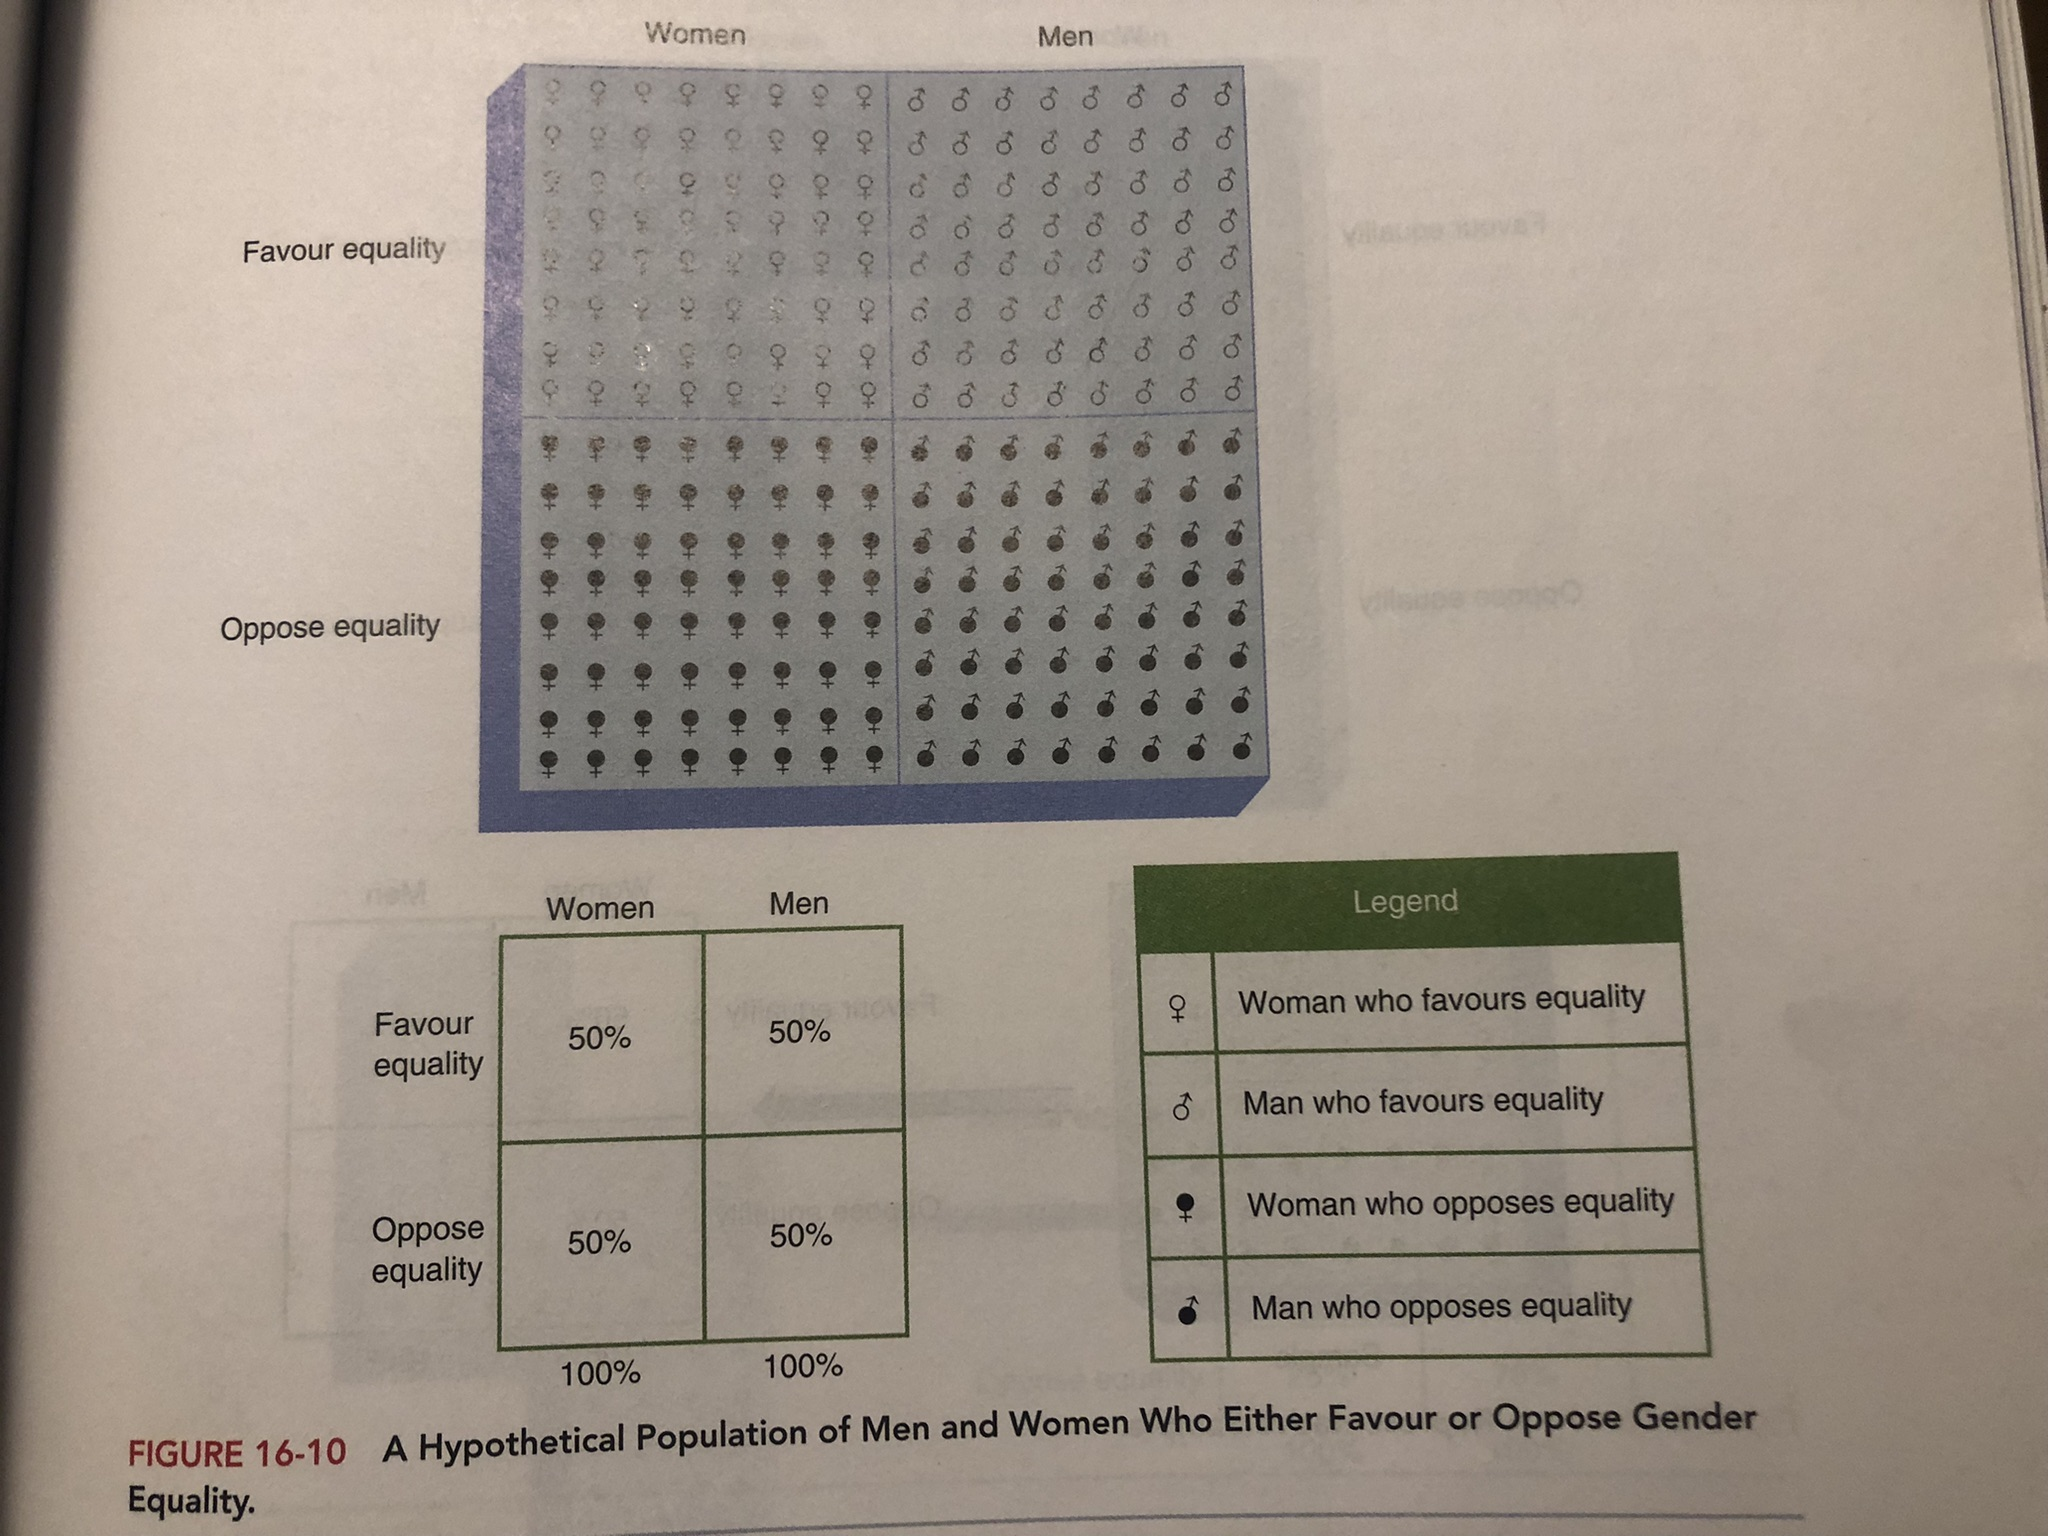
\includegraphics{/Users/visseho/OneDrive - UQAM/Cours/Images_cours/logique_test1.jpeg}
\caption{Figure 1}
\end{figure}

On voit que dans cette population, il y a un même pourcentage d'hommes
et de femmes qui sont favorables aux droits des femmes. Il n'y a donc
pas de relation entre le sexe et l'attitude par rapport à l'égalité.

Maintenant, tirons un échantillon aléatoire du quart de cette
population.

Le résultat nous donne ceci:

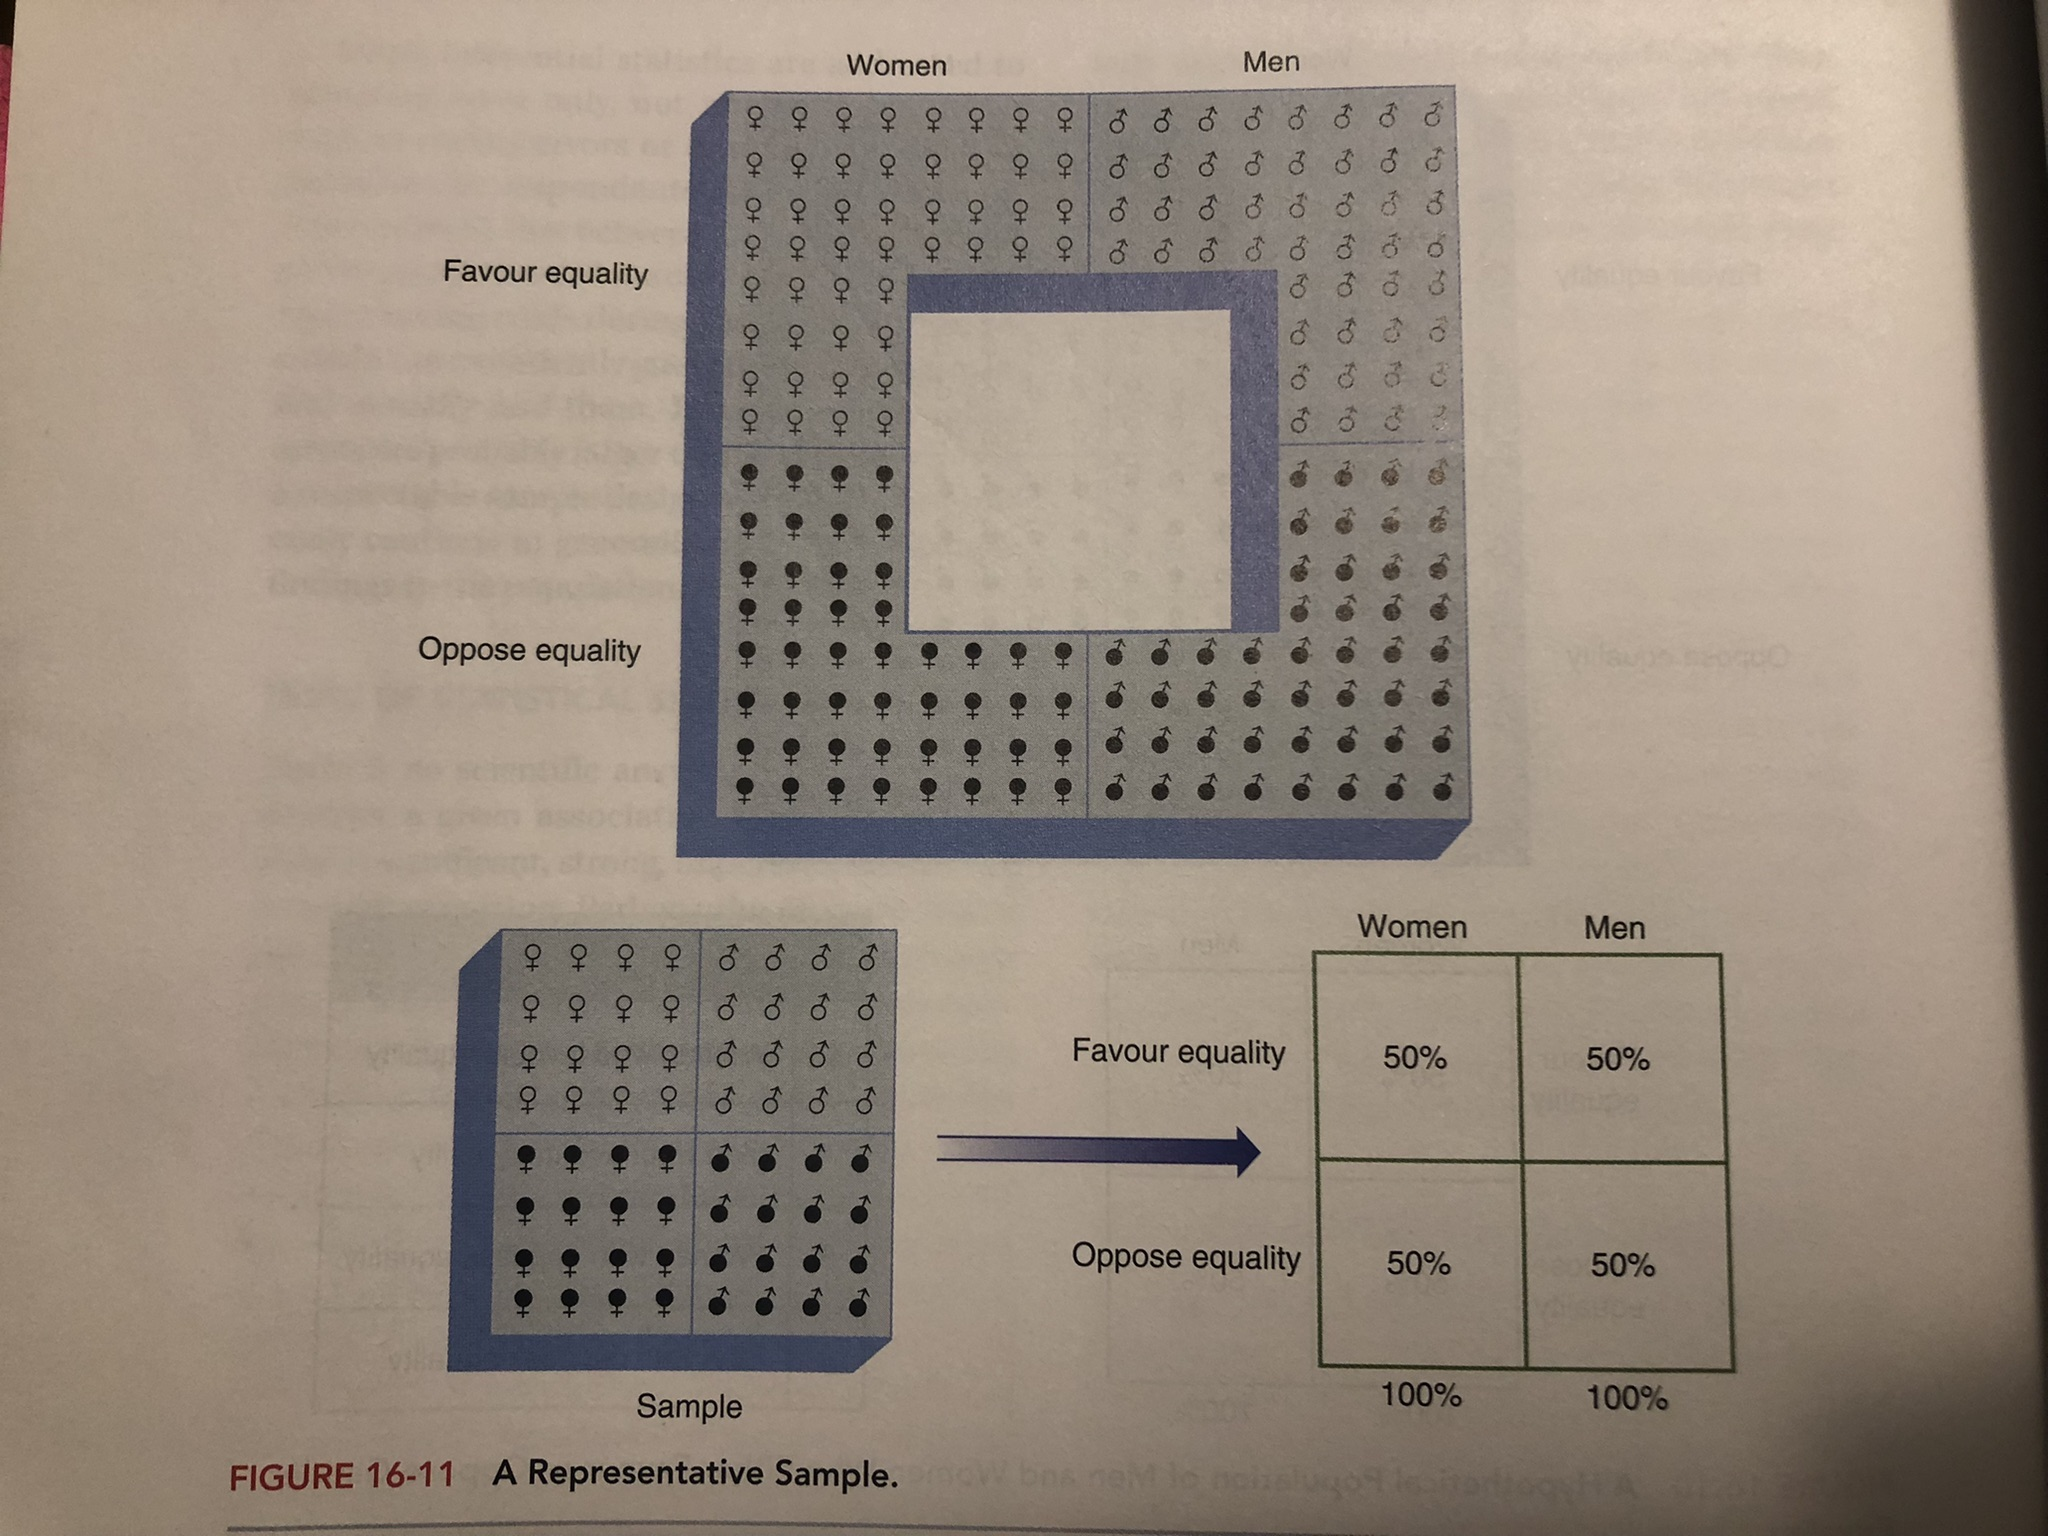
\includegraphics{/Users/visseho/OneDrive - UQAM/Cours/Images_cours/logique_test2.jpeg}

On peut voir clairement que cet échantillon est bien représentatif de la
population. Il n'existe pas de relation entre les deux variables. Cet
échantillon nous aurait ainsi permis de tirer une conclusion correcte
sur la population. A travers la logique de l'échantillonnage, nous
concluonerons qu'il n'y a pas de relation au sein de la population d'où
est tiré l'échantillon.

Il est évident aussi qu'on ne serait pas toujours tombé sur un
échantillon aussi parfait de la population. Il ne serait pas inhabituel
de trouver d'avoir 2 hommes de plus qui sont favorables aux droits des
femmes ou inversement.

Maintenant, regardons un autre échantillon:

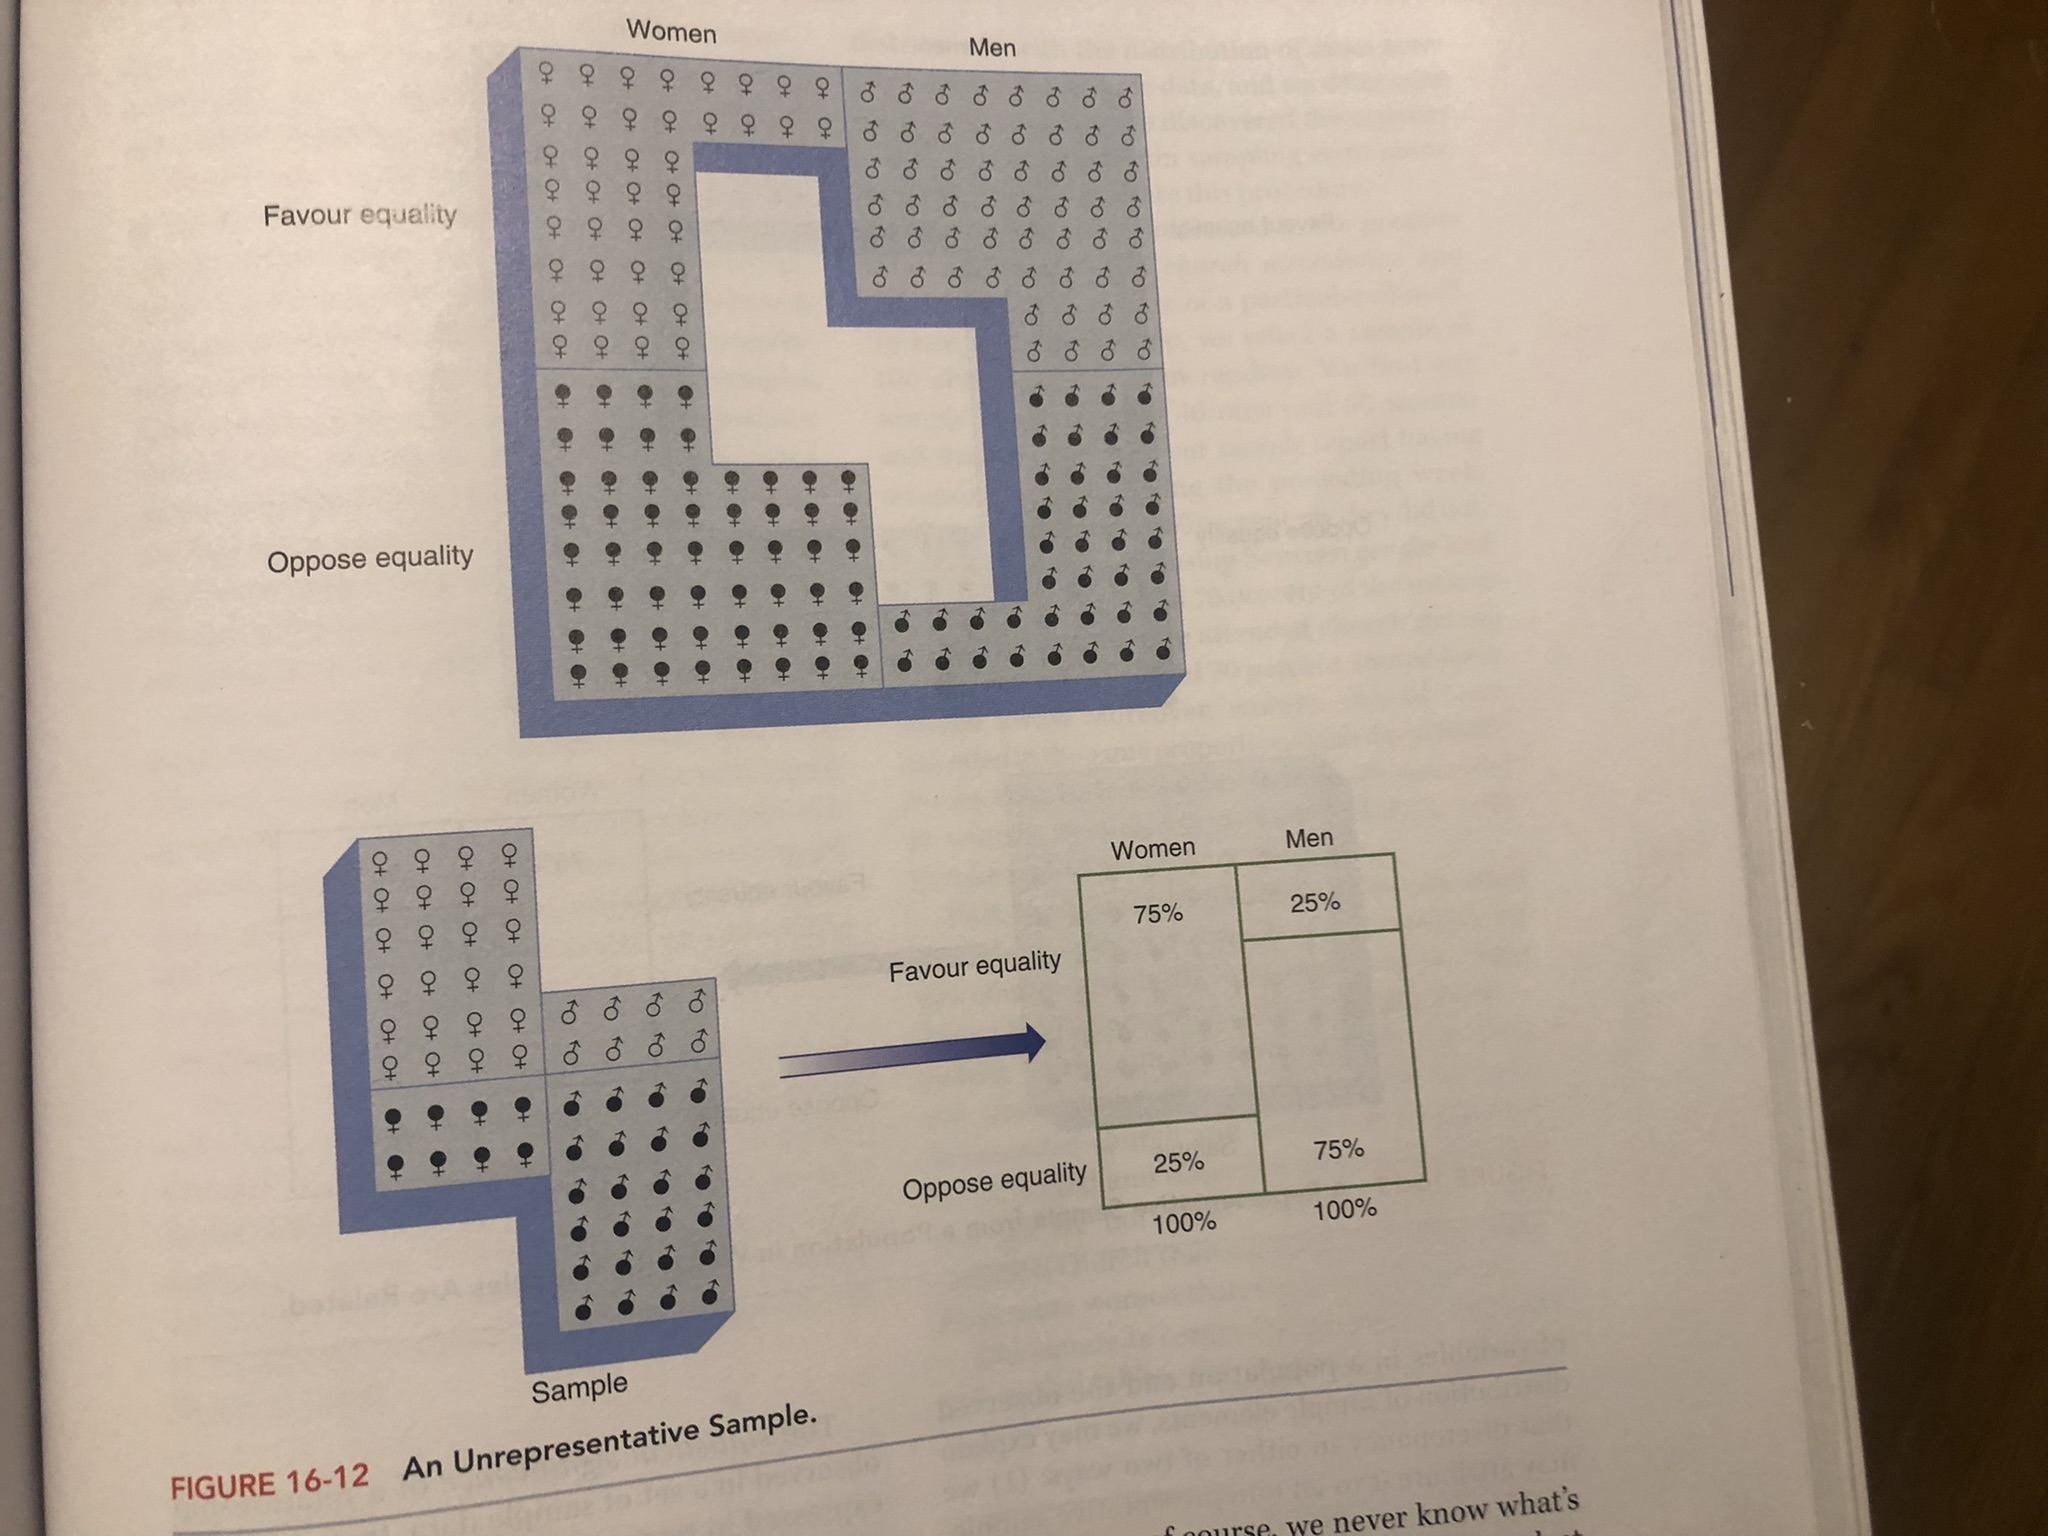
\includegraphics{/Users/visseho/OneDrive - UQAM/Cours/Images_cours/logique_test3.jpeg}

On voit que cet échantillon n'est pas représentatif de la population
précédente. Nous avons 3/4 des femmes qui sont favorables aux droits des
femmes contre 25\% des hommes. Si nous avons tiré un tel échantillon
dans une population où il n'y a pas de relation entre les deux
variables, nous serions fortement induits en erreur par l'analyse de
notre échantillon. Selon la logique de l'échantillonnage, il est très
peu probable que nous tirions un tel échantillon de notre population où
il n'y a pas d'association entre les deux variables. Il est donc plus
probable que cet échantillon provienne plutôt d'une population comme
celle-ci:

\begin{figure}
\centering
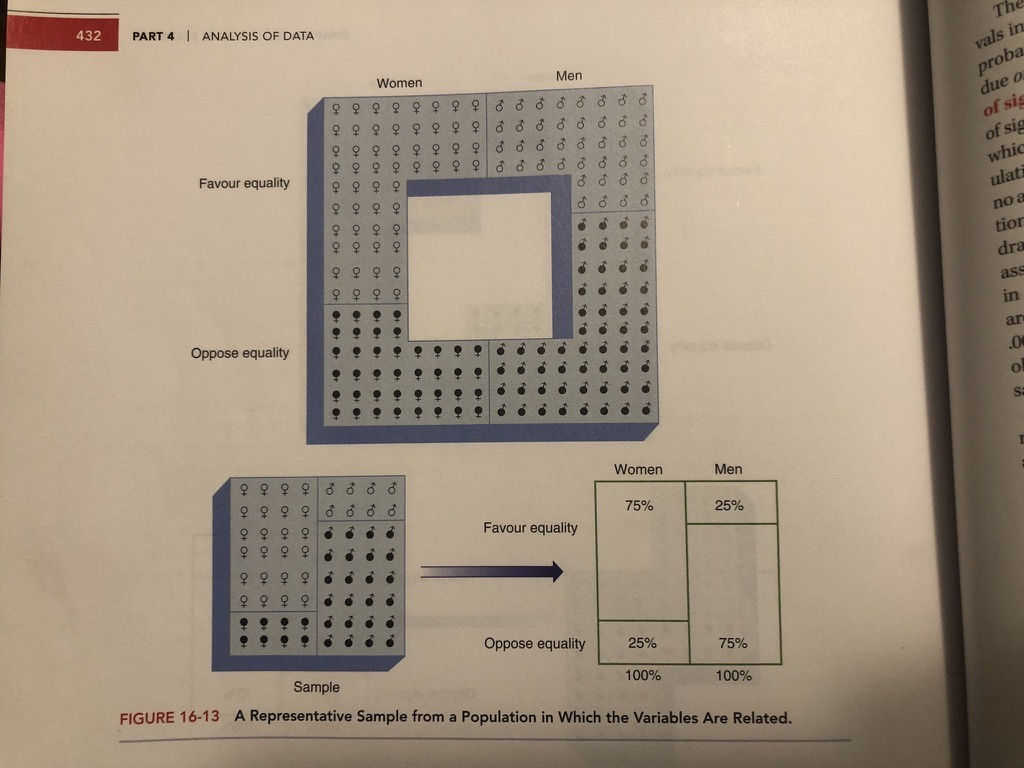
\includegraphics{/Users/visseho/OneDrive - UQAM/Cours/Images_cours/logique_test4.jpeg}
\caption{Figure 4}
\end{figure}

L'échantillon tiré de cette population nous indique aussi une relation
forte entre le sexe et l'opinion. Mais, cette fois-ci, cet échantillon
est représentatif de la population.

Dans les faits: 1. Nous ne connaissons pas la distribution dans la
population 2. Nous ne tirons qu'un seul échantillon.

Si nous faisons face à une association au sein de notre échantillon
alors que nous pensons qu'il n'y en a pas dans la population, nous
pouvons dire deux choses: 1. Soit que notre échantillon n'est pas
représentatif ou que 2. Soit qu'il existe bel et bien une association
entre les variables dans la population d'où est tirée notre échantillon.

\textbf{Que savons-nous sur les échantillons? }

Nous savons que si nous tirons plusieurs fois un échantillon dans une
population - Il y a de forte probabilité que l'échantillon soit
représentatif de la population - et de très faible probabilité que
l'échantillon ne soit pas représentatif.

\textbf{il existe une forte probabilité d'un faible degré de
non-représentativité et une faible probabilité d'un degré élevé de
non-représentativité}

La signification statistique d'une relation observée dans un ensemble de
données d'échantillon est donc toujours exprimée en termes de
probabilités. «Significatif au niveau de 0,05» signifie simplement que
la probabilité qu'une relation aussi forte que celle observée puisse
être attribuée à la seule erreur d'échantillonnage n'est pas supérieure
à 5 sur 100. En d'autres termes, si deux variables sont indépendantes
l'une de l'autre dans la population, et si 100 échantillons
probabilistes étaient sélectionnés dans cette population, pas plus de 5
de ces échantillons fourniraient une relation aussi forte que celle qui
a été observée.

0,05 est appelé le niveau de signification. Nous supposons qu'il n'y a
pas d'association entre les variables de la population, puis nous nous
demandons quelle proportion des échantillons tirés d'une telle
population produirait des associations au moins aussi importantes que
celles mesurées dans les données empiriques. Trois niveaux de
signification sont fréquemment utilisés dans les rapports de recherche :
0,05, 0,01, 0,001. Cela signifie, respectivement, que les chances
d'obtenir l'association mesurée à la suite d'une erreur
d'échantillonnage sont de 5/100, 1/100 et 1/1000.

\end{document}
